% day4_seg2_navaids/navaids_main.tex
\begin{frame}
\textbf{Day 4, Segment 2\\
Survey of Navaids\\
Topics}
 \begin{itemize}
 \item GPS
 \item Position Fixes
 \item Radar
 \item Doppler Velocity Sensor (DVS)
 \item External Tracking Aids
% \item Attitude References
 \item Digital Terrain Elevation Data (DTED)
\end{itemize}
\end{frame}
\begin{frame}
%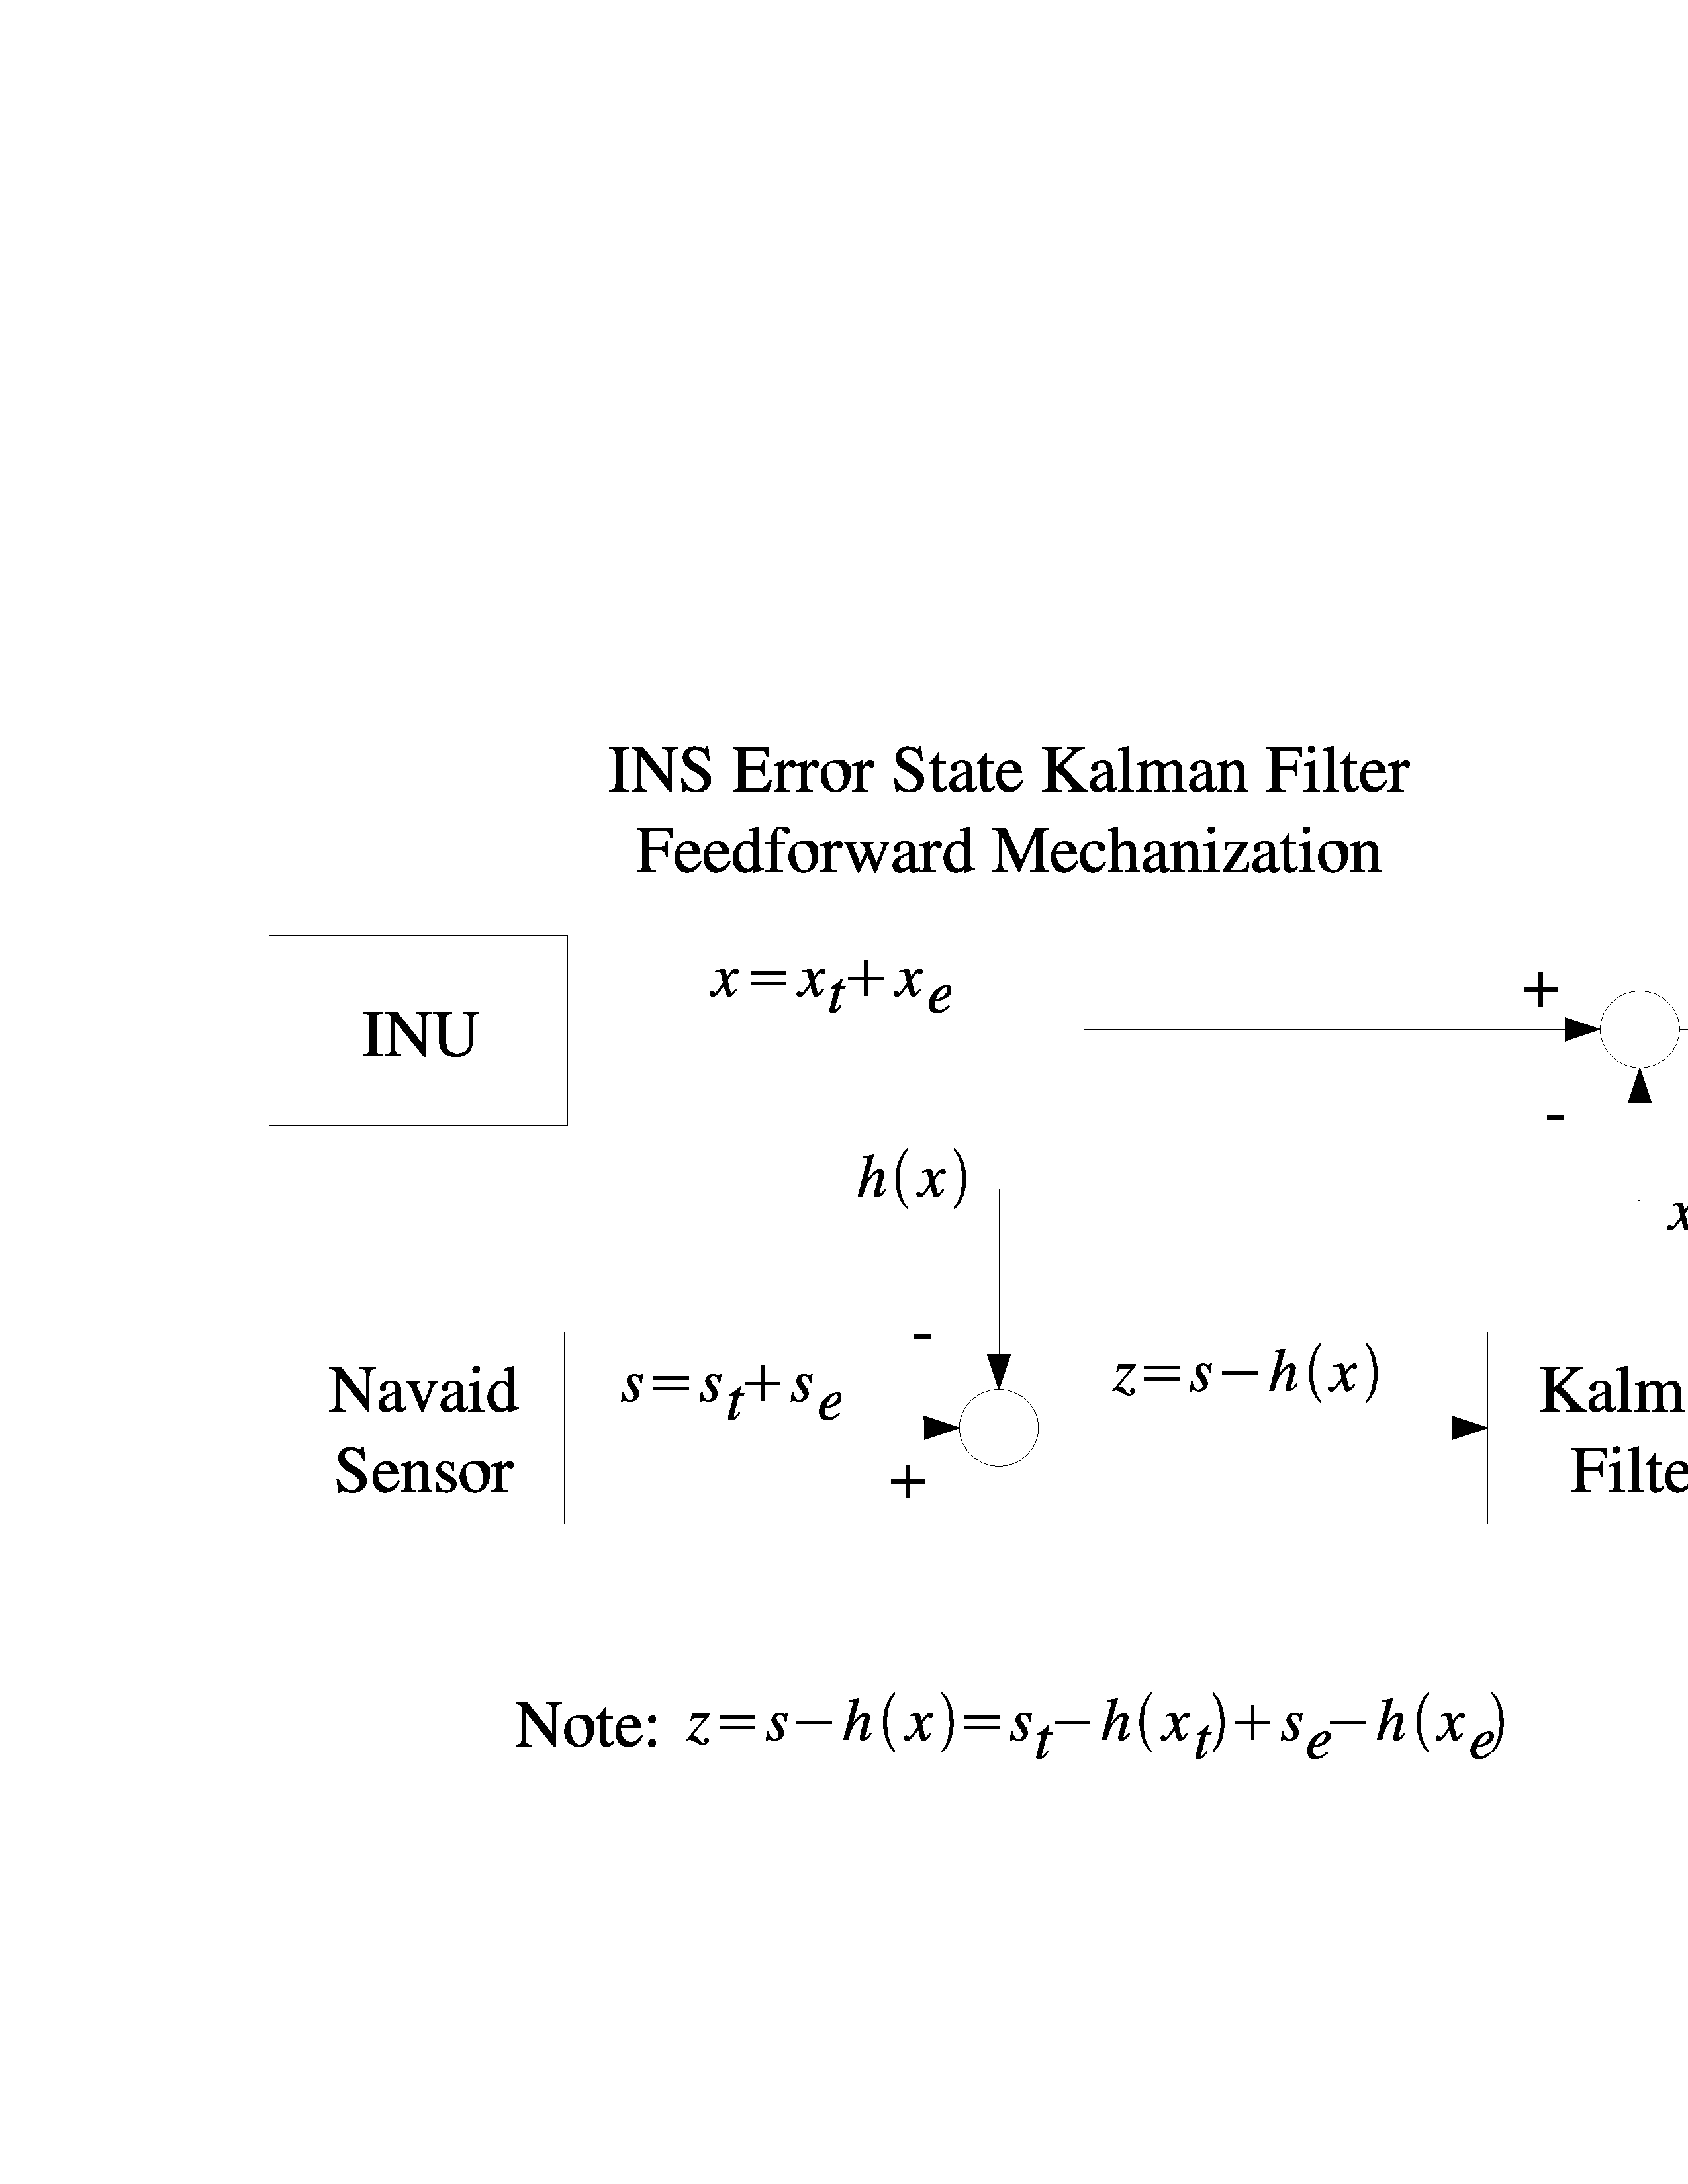
\includegraphics{day1_seg1_heuristic/feedforward.jpg}
\end{frame}

\begin{frame}
Navigation Aids (Navaids)
\begin{itemize}
  \item Measurement / Observation sources that aid in estimating INS error sources and dynamics
  \item Because we are interested in estimating INS errors, we use differencing to cancel out the whole state information
  \item INS outputs $x=x_t + x_e$, where $x_t$ is the true whole state information generated by INS, i.e., position, velocity, attitude, etc.
  \item Navaid sensor outputs $s=x_t+x_e$, where $x_t$ is once again the true quantities corrupted by sensor errors $x_e$.
\end{itemize} 
\end{frame}

\begin{frame}
Navigation Aids (Navaids)
\begin{itemize}
  \item Note that the navaid sensor usually only outputs part of the whole state vector, e.g., position and velocity, but not attitude (in the case of GPS)
  \item That's one reason why we have the $h$ function
  \item The INS signal is mapped by a linearized measurement function (or matrix) $h$ such that $h(x)=h(x_t) + h(x_e)$ and $h(x_t)=s_t$
\end{itemize} 
\end{frame}

\begin{frame}
Navigation Aids (Navaids)
\begin{itemize}
  \item Thus, we have
\begin{align*}
z&=s-h(x)\\
&=s_t + s_e - h(x_t) - h(x_e)\\
&=s_t - h(x_t) + s_e - h(x_e)\\
&=h(x_t) - h(x_t)+ s_e - h(x_e)\\
&=s_e - h(x_e)
\end{align*}
  \item Our measurement, therefore, is the difference between the navaid sensor errors and the INS errors
\end{itemize} 
\end{frame}

\begin{frame}
Navigation Aids (Navaids)
\begin{itemize}
  \item If $s_e$ is more than just white measurement noise, then we would need to model this vector in the filter according to known or assumed dynamics 
  \item Hence, sometimes adding a new navaid means adding new states to your filter

\end{itemize} 
\end{frame}

\begin{frame}
Navigation Aids (Navaids)
\begin{itemize}
  \item It is crucial to examine the innovations sequence for any non-white time correlations!
\[z_k-h\left[\stateest{k}{-}\right]=s_e(k)-h\left[(x_e(k)\right]-h\left[\stateest{k}{-}\right]\]
where we have added the index $k$ for clarity
 \item We should have $\expect{(z_k-h\left[\stateest{k}{-}\right])(z_j-h\left[\stateest{j}{-}\right])\trans}=0$ when $k\neq j$, which will in general be true provided $\expect{s_e(k)}=0$
 \item If this is not the case, then it is probably $s_e$ that is the culprit and you'd better start modeling!
\end{itemize} 
\end{frame}

\begin{frame}

\begin{itemize}
  \item The condition
\[\expect{(z_k-h\left[\stateest{k}{-}\right])(z_j-h\left[\stateest{j}{-}\right])\trans}=0
\]
says that the innovations sequence is uncorrelated in time.
  \item Recall that the innovations sequence is $\nu_k=z_k-h\left[\stateest{k}{-}\right]$
  \item Thus, we should have $\expect{\nu_k \nu_j\trans}=0$
  \item This means that the optimal estimator $\stateest{k}{+}$ always makes optimal use of the new information provided by $\nu_k$
\end{itemize} 
\end{frame}


% day4_seg2_navaids/gps.tex
\begin{frame}
GPS: The Global Positioning System
 \begin{itemize}
 \item 24+ satellites orbiting at 10,900 miles above surface
 \item Three Segments: Control, Space, User
 \item Time-tagged signals and known satellite position enable calculation of signal time of flight and hence range traversed from satellite to receiver
 \item Range to four satellites required to determine time plus three position coordinates
\end{itemize}
\end{frame}

\begin{frame}
GPS: The Global Positioning System
\begin{itemize}
  \item Satellites have precise atomic clocks
  \item User set receiver has less precise clock
  \item Time is of the essence:  comparing satellite-generated time-tag with user clock time of arrival determines transit time
  \item Note that user clock can be a source of systematic error
\end{itemize} 
\end{frame}

\begin{frame}
GPS: The Global Positioning System
\begin{itemize}
  \item Three types of navaid coupling:
  \begin{itemize}
	\item Loose coupling
    \item Tight coupling
    \item Deep coupling
  \end{itemize} 
\end{itemize} 
\end{frame}

\begin{frame}
Loosely-Coupled GPS
\begin{itemize}
  \item GPS receiver-generated position and velocity are differenced with INS position and velocity
  \item GPS position and velocity are generally pre-filtered (with a Kalman filter) before being used in inertial filter
  \item GPS position and velocity are also composite quantities from all satellites
  \item Least accurate approach to using GPS as a navaid
\end{itemize} 
\end{frame}

\begin{frame}
Loosely-Coupled GPS
\begin{itemize}
  \item The GPS receiver does not have the advantage of using inertial information to completely separate process noise from measurement noise
  \item Simplifies Kalman integration: Don't necessarily have to model GPS receiver clock errors (assume receiver has already done so)
\end{itemize} 
\end{frame}

\begin{frame}
Tightly-Coupled GPS
\begin{itemize}
  \item Pseudorange and delta pseudorange for each individual satellite are direct measurements presented to the filter
  \item Contains only measurement noise, not receiver filter's model of process noise 
  \item Gives INS filter more fine-grained control over GPS measurements
  \item Higher accuracy
\end{itemize} 
\end{frame}

\begin{frame}
Deeply-Coupled
\begin{itemize}
  \item Uses high-rate inertial data to aid in code and carrier phase tracking loops
  \item Most accurate solution when combined with tightly-coupled INS filter as well
\end{itemize} 
\end{frame}

\begin{frame}
GPS Errors
\begin{itemize}
  \item Ephemeris data: Satellite's reported position can be in error
  \item Satellite clock:  Negligible since SA (selective availability) has been turned off
  \item Ionosphere:  Pseudorange errors caused by free electrons in the ionosphere
\end{itemize} 
\end{frame}

\begin{frame}
GPS Errors (cont)
\begin{itemize}
  \item Troposphere: Pseudorange errors casued by temperature, pressure, humidity influences on the speed of light
  \item Multipath:  Errors casued by locking on to reflected signals
  \item Receiver Noise: Errors caused by receiver's thermal noise and software inaccuracies
\end{itemize} 
\end{frame}

\begin{frame}
\begin{center}
%\begin{tabular}{|c|p{2.5in}|p{2.5in} |} \hline
 \begin{tabular}{|p{3in}|p{1.5in}|p{1.5in}|} \hline
 % after \\ : \hline or \cline{col1-col2} \cline{col3-col4} ...
  \textbf{Error Source} & \textbf{C/A-Code Error Budget (meters)} & \textbf{P-Code Error Budget (meters)} \\ \hline
Multipath & 12.0 & 1.2 \\ \hline
Receiver Noise / Software & 11.1 & 1.1 \\ \hline
Ionosphereic Delays & 9.0 & 3.1 \\ \hline
Satellite Clock and  Ephemeris Errors & 3.9 & 3.9 \\ \hline
Tropspheric Delays & 2.0 & 2.0 \\ \hline
\end{tabular}
\end{center}
\end{frame}

\begin{frame}
Using Loosely-Coupled GPS Measurements
\begin{itemize}
  \item Position
	\begin{itemize}
		\item Form primary GPS position observation by subtracting Kalman-corrected INS reference position from raw GPS position
		\item Next, the innovation (or measurement residual) is formed by subtracting off the extrapolated state estimate of position error
		\item Extrapolated position error estimate needs to compensate for accumulated velocity error during Kalman cycle (or some fraction thereof) 
	\end{itemize}
\end{itemize} 
\end{frame}

\begin{frame}
An example (JOVIAL) from a transport aircraft navigation filter:
\end{frame}
\begin{verbatim}
  165  COMPUTE RESIDUALS 
  166      RESIDUALS(1) = Y'KAL'OBS(INU,1) * OBS'COUNT'SCALER - SVVAR(1)
  167 	- 5.0 * SVVAR(4);
  168      RESIDUALS(2) = Y'KAL'OBS(INU,2) * OBS'COUNT'SCALER - SVVAR(2)
  169 	- 5.0 * SVVAR(5);
  170      RESIDUALS(3) = Y'KAL'OBS(INU,7) * OBS'COUNT'SCALER - SVVAR(3)     
  171         - 5.0 * SVVAR(6);

\end{verbatim}

\begin{frame}
GPS Velocity Measurements
\begin{itemize}
  \item Based on carrier phase measurements in receiver
  \item Generally independent of position measurements
  \item Observation is once again difference between Kalman-compensated INS reference velocity and GPS-indicated velocity
\end{itemize} 
\end{frame}

\begin{frame}
GPS Measurment Noise Covariance
\begin{itemize}
  \item Based on EHE (estimated horizontal error) and EVE (estimated vertical error)
  \item These numbers highgly dependent on GDOPs
\end{itemize} 
\end{frame}

\begin{frame}
Geometric Dillution of Precision (GDOP)
\begin{itemize}
  \item Satellites are not geostationary
  \item H matrix is time-varying
  \item Observability varies with time
  \item $GDOP=\sqrt{\text{tr}\left(H\trans H\right)^{-1}}$
\end{itemize} 
\end{frame}


\begin{frame}
GDOP Chimney
\begin{itemize}
  \item Large DGOP is bad; normal values 3-5
  \item Singularity periods of time (about 1 hr) when GDOP values spike upward with a peak as much as 1000
  \item GDOP 50 $\approx$ 500 m position error
  \item Chimney's effects should be less acute if receiver has enough channels to track many satellites and to handle constellation changes
\end{itemize} 
\end{frame}


% day4_seg2_navaids/posfix.tex
\begin{frame}
Position Fix
 \begin{itemize}
 \item Overfly Fix
 \item Known location
 \item Delta formed between overfly location and indicated, Kalman-compensated INS position
 \item Usually a one-shot opportunity, i.e., not periodic like GPS
\end{itemize}
\end{frame}

% day4_seg2_navaids/radar.tex
\begin{frame}
Radar Fixes
 \begin{itemize}
 \item Instantaneous azimuth and elevation angles to a target of known latitude and longitude
 \item Or converted to local Cartesian coordinates (north, east, and altitude)
 \item Amount of cursor movement required to align curson with target yields position fix delta
 \item Otherwise, processed in filter like GPS or visual position fix
\end{itemize}
\end{frame}

% day4_seg2_navaids/dvs.tex
\begin{frame}
Doppler Velocity Sensor (DVS)
 \begin{itemize}
 \item DVS provides genuine velocity measurement with respect to ground
 \item DVS provides heading and drift velocities $V_H$ and $V_D$
 \item Nonlinear measurement relationship to INS-indicated velocities $V_x$ and $V_y$ and platform azimuth $\beta$:
\end{itemize}
\begin{align*}
V_H &= -V_x\sin\beta + V_y\cos\beta\\
V_D &=  V_x\cos\beta + V_y\sin\beta
\end{align*}
\end{frame}

\begin{frame}
DVS
\begin{itemize}
  \item Relationship between $(V_x,V_y)$ and $(V_H,V_D)$ is non-linear $h$
  \item To generate a linearized $H$ matrix we compute partial derivatives (Jacobians) to yield:
\[H=
\begin{bmatrix}
0&-\sin\beta&0&0&\cos\beta&0&0&0&-V_x\cos\beta - V_y\sin\beta\\
0&\cos\beta&0&0&\sin\beta&0&0&0&-V_x\sin\beta + V_y\cos\beta
\end{bmatrix}
\]
for a canonical 9-state filter.
\end{itemize} 
\end{frame}

% day4_seg2_navaids/tracking.tex
\begin{frame}
External Tracking Aids
 \begin{itemize}
 \item External platform tracks your vehicle and sends position / velocity info (JTIDS) 
 \item Bearing and distance measurments
	\begin{itemize}
		\item VOR, DME, TACAN
	\end{itemize}
\end{itemize}
\end{frame}

%% day4_seg2_navaids/att.tex
\begin{frame}
Attitude References
 \begin{itemize}
 \item 
 \item
 \item
\end{itemize}
\end{frame}

% day4_seg2_navaids/dted.tex
\begin{frame}
Digital Terrain Elevation Data (DTED)
 \begin{itemize}
 \item Published by National Geospatial Intelligence Agency (NGA)
	\begin{itemize}
		\item formerly NIMA, formerly DMA
	\end{itemize}
 \item 1 deg geocells of terrain height for each lat/long pair
 \item DTED Levels 0,1,2
\end{itemize}
\end{frame}

\begin{frame}
DTED
\begin{itemize}
  \item As navaid, a trail of radar altimeter measurements are stored
  \item Trail is correlated with DTED to determine offset
  \item SITAN, TERPROM
\end{itemize} 
\end{frame}

%% day4_seg2_navaids/exercises.tex
\begin{frame}
Exercises
 \begin{itemize}
 \item
 \item
 \item
\end{itemize}
\end{frame}

